\documentclass[12pt,a4paper]{article}

\usepackage{german}      % Deutsche TeX-Eigenheiten
%\usepackage{isolatin1}   % Eingabekodierung mit Umlauten...

\usepackage{makeidx}
\makeindex            % damit eine Indexdatei angelegt wird

\usepackage{graphicx}

\usepackage{amsmath}  % allgemeine Mathe-Erweiterungen
\usepackage{amssymb}  % Symbole und Schriftarten
\usepackage{amsthm}   % erweiterte Theorem-Umgebungen

\usepackage{mathrsfs}  % gibt den Befehl "\mathscr{}" für schöne

\usepackage[noframe]{showframe}
\usepackage{framed}
\renewenvironment{shaded}{%
	\def\FrameCommand{\fboxsep=\FrameSep \colorbox{shadecolor}}%
	\MakeFramed{\advance\hsize-\width \FrameRestore\FrameRestore}}%
{\endMakeFramed}
\definecolor{shadecolor}{gray}{0.75}

\newcommand\underrel[2]{\mathrel{\mathop{#2}\limits_{#1}}}

\begin{document}
\section{L'Hospital}
\textbf{1. Regel} Bei \textcolor{red}{$\frac{0}{0}$}:$\lim\limits_{x\rightarrow x_0}\frac{f(x)}{g(x)}=\lim\limits_{x\rightarrow x_0}\frac{f'(x)}{g'(x)}$\\
\textbf{2. Regel} Bei \textcolor{red}{$\frac{a}{\infty}$}:$\lim\limits_{x\rightarrow x_0}\frac{f(x)}{g(x)}=\lim\limits_{x\rightarrow x_0}\frac{f'(x)}{g'(x)}$\\
Umformen bei: $0\cdot\infty, 0^0,\infty,1^\infty,\infty-\infty$\\
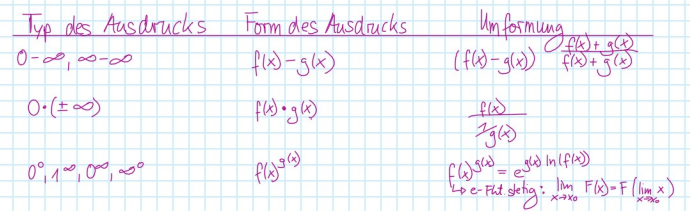
\includegraphics[width=0.8\textwidth]{Bilder/Zusfa/1.png}
\section{Taylor}
Formel:
$$
\begin{matrix}
f(x)=\underbrace{f(x_0)+\frac{f'(x_0)}{1!}\left(x-x_0\right)+\frac{f''(x_0)}{2!}\left(x-x_0\right)^2...+\frac{f^{(n)}(x_0)}{n!}\left(x-x_0\right)^n}_{\text{Taylorpolynom n-ter Ordnung (Hauptteil)}}\\
\\
+\underbrace{\frac{f^{(n+1)}(\xi)}{\left(n+1\right)!}\left(x-x_0\right)^{n+1}}_{R_n \text{Restglied von Lagrange}}
\end{matrix}
$$

Entwicklungspunkt $x_0$ = beliebig, aber fest aus Intervall\\
Zwischenstelle $\xi$ liegt zwischen x und $x_0$, kann also kleiner als x oder auch größer sein.\\
\subsubsection{Fehlerabschätzung}
worst case: $\xi$ zwischen $x_0$ und $x$ so wählen, dass $|R_n(x)|$ größtmöglich wird.\\
$$
\begin{matrix}
\Rightarrow\left|f(x)-P_n(x)\right|=\left|R_n(x)\right| &=& \left|\frac{1}{\left(n+1\right)!}f^{(n+1)}(\xi)\left(x-x_0\right)^{n+1}\right| \\
\\
&=& \frac{1}{\left(n+1\right)!}\left|\left(x-x_09\right)^{n+1}\right|\left|f^{(n+1)}(\xi)\right| \\
\\
&\leq& \frac{1}{\left(n+1\right)!}\left|\left(x-x_09\right)^{n+1}\right| M \\
\end{matrix}
$$
\newpage
Man sieht:\\
1. Je größer das n, dest kleiner wird der Faktor $1\frac{1}{(1-n)!}$\\
auf Deutsch: mit Großerem n wird die approximation besser\\
2. Je weiter das x von $x_0$ weg liegt, desto größer wird der Bertrag $x-x_0$, \\
desto mehr Einfluss hat der Term auf die Genauigkeit\\
\section{Reihen}
Die Folge $s_n$ nennt man die zur Folge $a_k$ gehörige unendliche
Reihe. Das n-te Glied heißt n-te Partialsumme.
$s_n=\sum\limits_{k=1}^{n}a_k$
Falls die Folge $s_n$ der Partialsummen keinen Grenzwert
besitzt, nennt man die Reihe \textbf{divergent}.
Die Reihe heißt \textbf{konvergent}, wenn $s_n$ konvergiert. 
\\Dann setzt man
$s=\lim\limits_{n\rightarrow \infty}s_n=\lim\limits_{n\rightarrow \infty}\sum\limits_{k=1}^{n}a_k=\sum\limits_{k=1}^{\infty}a_k$
\\Im Falle der Konvergenz sagt man die Reihe $\sum\limits_{k=1}^{\infty}a_k$ ist \textbf{konvergent} und nennt $s$ den Grenzwert die Simme der unendlichen Reihe. 
\subsection{Geometrische Reihe}
$\sum\limits_{k=0}^{\infty}q^k=\frac{1}{1-q},|q|<1$
\\
Für \textcolor{red}{$|q|>1$} wächst der Term $q_n+1$ für $n\rightarrow\infty$ betragsmäßig unbeschränkt,\\ so dass \textbf{Divergenz} der Folge $s_n$ und somit der Reihe vorliegt.
\\
\\
Im Fall \textcolor{red}{$q=1$} gilt für die Partialsumme $s_n=n+1$.\\Damit liegt \textbf{Divergenz} der Reihe vor.
\\
\\
Im Fall \textcolor{red}{$|q|<1$} strebt $q_n+1$ gegen den Grenzwert 0 und die Reihe ist \textbf{konvergent}.
\\
\\
Im Fall \textcolor{red}{$q=-1$} wechselt $s_n$ fortlaufend zwischen den Werten 1 und 0, d.h. es liegt \textbf{Divergenz} vor
\\
\\
\subsection{harmonische Reihe}
$a_k=\frac{1}{\phantom{...}\underbrace{k}_{>0}\phantom{...}}\Rightarrow s_n=a_1+a_2+...+a_n=\overbrace{1+\frac{1}{2}+...+\frac{1}{n}}^{harmonische Reihe}$\\
Die harmonische Reihe ist \textbf{divergent}.
\\\underline{\textbf{\textcolor{red}{Divergenzkriterium:}}}
Falls die Folge $a_k$ \textbf{nicht} gegen Null konvergiert, ist die
unendliche Reihe\\ 
$\sum\limits_{k=1}^{\infty}a_k$ \textbf{divergent.}
Notwendig für die Konvergenz einer Reihe $\sum\limits_{k=1}^{\infty}a_k$ ist die Bedingung, dass die Folge $a_k$
eine \underline{Nullfolge} ist, also $\lim\limits_{k\rightarrow\infty}a_k=0$
\section{Absolute und bedingte Konvergenz von Reihen, Konvergenzkriterien}
Summen und Vielfache konvergenter Reihen ergeben wieder eine konvergente Reihe.
\subsection{bedingte/ absolute Konvergenz}
Die Reihe $\sum\limits_{k=1}^{\infty}a_k$ heißt \textbf{absolut konvergent}, wenn die Reihe der Beträge konvergent ist $\sum\limits_{k=1}^{\infty}|a_k|$
\\
Eine konvergente Reihe, welche nicht absolut konvergent ist, heißt \textbf{bedingt konvergent}.
\\Eine \textbf{absolut konvergente} Reihe ist auch \textbf{(bedingt) konvergent}, die Umkehrung ist i.a. falsch.
\\\underline{\textbf{\textcolor{red}{Majorantenkriterium:}}}\\
$\sum\limits_{k=1}^{\infty}c_k$ konvergente Reihe mit nichtnegativen Gliedern und es gelte $|a_k|\leq c_k$ für alle $k\geq m (fest)$\\
Dann ist die Reihe $\sum\limits_{k=1}^{\infty}a_k$ \textbf{absolut konvergent}.
Bsp:\\
$\sum\limits_{k=1}^{\infty}\frac{k}{k^3+k} \Rightarrow k$ ausklammern $= \frac{k}{k(k^2+1)}=\frac{1}{k^2+1}$
\\Die Reihe verhält sich wie $\sum\limits_{k=1}^{\infty}\frac{1}{k^2}$, sollte daher konvergieren. Begründung:
\\Aus $k^2+1 \geq k^2$ folgt: $\frac{k}{\underbrace{k^3+k}_{=|a_k}}=\frac{1}{k^2+1}\leq \frac{1}{\underbrace{k^2}_{=c_k}}$ 
\\Da nun die Reihe $\sum\limits_{k=1}^{\infty}c_k=\sum\limits_{k=1}^{\infty}\frac{1}{k^2}$ konvergiert, konvergiert auch die Reihe $\sum\limits_{k=1}^{\infty}a_k=\sum\limits_{k=1}^{\infty}\frac{k}{k^3+k}$
\\\underline{\textbf{\textcolor{red}{Minorantenkriterium:}}}\\
$\sum\limits_{k=1}^{\infty}d_k$ divergente Reihe mit nichtnegativen Gliedern und es gelte $a_k\geq d_k$ für alle $k\geq m (fest)$\\
Dann ist die Reihe $\sum\limits_{k=1}^{\infty}a_k$ \textbf{divergent}.
\\Bsp:\\
$\sum\limits-{k=1}^{\infty}\frac{1}{2k-1}$ wächst ähnlich wie $\sum\limits_{k=1}^{\infty}\frac{1}{2k}$\\
Da nun die harmonische Reihe $\sum\limits_{k=1}^{\infty}\frac{1}{k}$ divergiert, divergiert auch die Reihe $\sum\limits_{k=1}^{\infty}\frac{1}{2k}$ und damit auch $\sum\limits_{k=1}^{\infty}\frac{1}{2k-1}$
\\$2k-1\leq 2k \leftrightarrow \frac{1}{\underbrace{2k-1}_{a_k}}\geq \frac{1}{\underbrace{2k}_{=c_k}}$
\end{document} 